%%
%% Automatically generated file from DocOnce source
%% (https://github.com/hplgit/doconce/)
%%
%%


%-------------------- begin preamble ----------------------

\documentclass[%
twoside,                 % oneside: electronic viewing, twoside: printing
final,                   % or draft (marks overfull hboxes, figures with paths)
10pt]{article}

\listfiles               % print all files needed to compile this document

\usepackage{relsize,makeidx,color,setspace,amsmath,amsfonts}
\usepackage[table]{xcolor}
\usepackage{bm,microtype}

\usepackage{graphicx}

\usepackage{fancyvrb} % packages needed for verbatim environments

\usepackage{minted}
\usemintedstyle{default}

\usepackage[T1]{fontenc}
%\usepackage[latin1]{inputenc}
\usepackage{ucs}
\usepackage[utf8x]{inputenc}

\usepackage{lmodern}         % Latin Modern fonts derived from Computer Modern

% Hyperlinks in PDF:
\definecolor{linkcolor}{rgb}{0,0,0.4}
\usepackage{hyperref}
\hypersetup{
    breaklinks=true,
    colorlinks=true,
    linkcolor=linkcolor,
    urlcolor=linkcolor,
    citecolor=black,
    filecolor=black,
    %filecolor=blue,
    pdfmenubar=true,
    pdftoolbar=true,
    bookmarksdepth=3   % Uncomment (and tweak) for PDF bookmarks with more levels than the TOC
    }
%\hyperbaseurl{}   % hyperlinks are relative to this root

\setcounter{tocdepth}{2}  % number chapter, section, subsection

% Tricks for having figures close to where they are defined:
% 1. define less restrictive rules for where to put figures
\setcounter{topnumber}{2}
\setcounter{bottomnumber}{2}
\setcounter{totalnumber}{4}
\renewcommand{\topfraction}{0.85}
\renewcommand{\bottomfraction}{0.85}
\renewcommand{\textfraction}{0.15}
\renewcommand{\floatpagefraction}{0.7}
% 2. ensure all figures are flushed before next section
\usepackage[section]{placeins}
% 3. enable begin{figure}[H] (often leads to ugly pagebreaks)
%\usepackage{float}\restylefloat{figure}

\usepackage[framemethod=TikZ]{mdframed}

% --- begin definitions of admonition environments ---

% --- end of definitions of admonition environments ---

% prevent orhpans and widows
\clubpenalty = 10000
\widowpenalty = 10000

% --- end of standard preamble for documents ---


% insert custom LaTeX commands...

\raggedbottom
\makeindex

%-------------------- end preamble ----------------------

\begin{document}



% ------------------- main content ----------------------

% Slides for PHY981


% ----------------- title -------------------------

\thispagestyle{empty}

\begin{center}
{\LARGE\bf
\begin{spacing}{1.25}
Computing in Science Education (CSE): Integrating a computational perspective in the basic science education
\end{spacing}
}
\end{center}

% ----------------- author(s) -------------------------

\begin{center}
{\bf Morten Hjorth-Jensen, National Superconducting Cyclotron Laboratory and Department of Physics and Astronomy, Michigan State University, East Lansing, MI 48824, USA {\&} Department of Physics, University of Oslo, Oslo, Norway${}^{}$} \\ [0mm]
\end{center}

    \begin{center}
% List of all institutions:
\end{center}
    
% ----------------- end author(s) -------------------------

\begin{center} % date
February 26, 2015
\end{center}

\vspace{1cm}


% !split
\subsection*{People and links}

% --- begin paragraph admon ---
\paragraph{}
\begin{itemize}
\item Hans Petter Langtangen, Computer Science

\item Knut Morken, Mathematics

\item Anders Malthe Sorensen and Arnt Inge Vistnes, Physics

\item Tom Lindstrom, Mathematics

\item Oyvind Ryan, Mathematics

\item Solveig Kristensen, Dean of Education

\item Hanne Solna, Director of studies

\item \href{{http://www.mn.uio.no/english/about/collaboration/cse/}}{\nolinkurl{http://www.mn.uio.no/english/about/collaboration/cse/}}

\item \href{{http://www.mn.uio.no/english/about/collaboration/cse/national-group/computing-in-science-education.pdf}}{\nolinkurl{http://www.mn.uio.no/english/about/collaboration/cse/national-group/computing-in-science-education.pdf}}
\end{itemize}

\noindent
% --- end paragraph admon ---




% !split
\subsection*{More links}

% --- begin paragraph admon ---
\paragraph{}
\begin{itemize}
\item Python and our first programming course, first semester \href{{http://www.uio.no/studier/emner/matnat/ifi/INF1100/h14/}}{course}. Excellent new textbook by Hans Petter Langtangen, click here for the \href{{http://www.amazon.com/Scientific-Programming-Computational-Science-Engineering-ebook/dp/B00DGER1NQ/ref=sr_1_2?ie=UTF8&qid=1425382942&sr=8-2&keywords=langtangen}}{textbook} or the \href{{http://hplgit.github.io/primer.html/doc/web/index.html}}{online version}

\item Mathematical modelling course, first semester \href{{http://www.uio.no/studier/emner/matnat/math/MAT-INF1100/h14/}}{course}. Textbook by Knut Morken to be published by Springer.

\item Mechanics, second semester \href{{http://www.uio.no/studier/emner/matnat/fys/FYS-MEK1100/v12/}}{course}. New textbook by Anders Malthe-Sorenssen, in press by Springer, Undergraduate Lecture Notes in Physics

\item Computational Physics I, fifth semester \href{{http://www.uio.no/studier/emner/matnat/fys/FYS3150/h14/}}{course}. Textbook to be published by IOP in 2015, with \href{{http://www.uio.no/studier/emner/matnat/fys/FYS3150/h14/undervisningsmateriale/Lecture%20Notes/lecture2014.pdf}}{online version}.
\end{itemize}

\noindent
% --- end paragraph admon ---





% !split
\subsection*{Wouldn't it be cool if your mechanics students could reproduce results in a PRL?}

% --- begin paragraph admon ---
\paragraph{}


% inline figure
\centerline{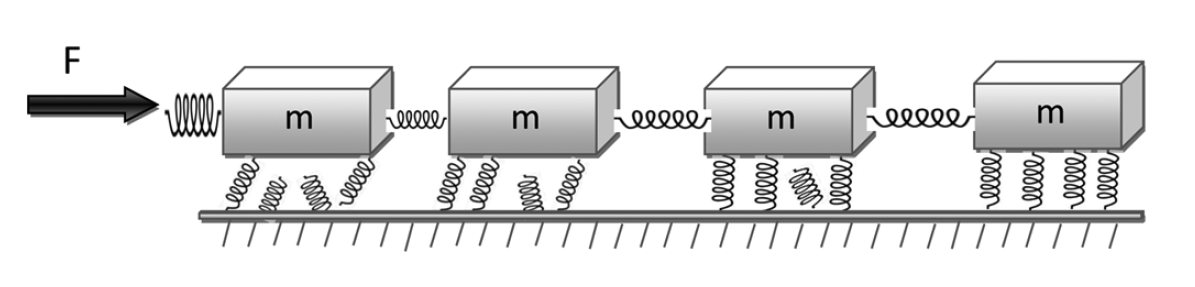
\includegraphics[width=0.5\linewidth]{figures/prl1.png}}



Grand challenge project in FYS-MEK1100 (Mechanics), Second Semester: a friction model to be solved as coupled ODEs. And find problems with the article?
% --- end paragraph admon ---



% --- begin paragraph admon ---
\paragraph{}


% inline figure
\centerline{
\includegraphics[width=0.5\linewidth]{figures/prl2.png}}
% --- end paragraph admon ---




% !split
\subsection*{Funny aside?}

% --- begin paragraph admon ---
\paragraph{}


% inline figure
\centerline{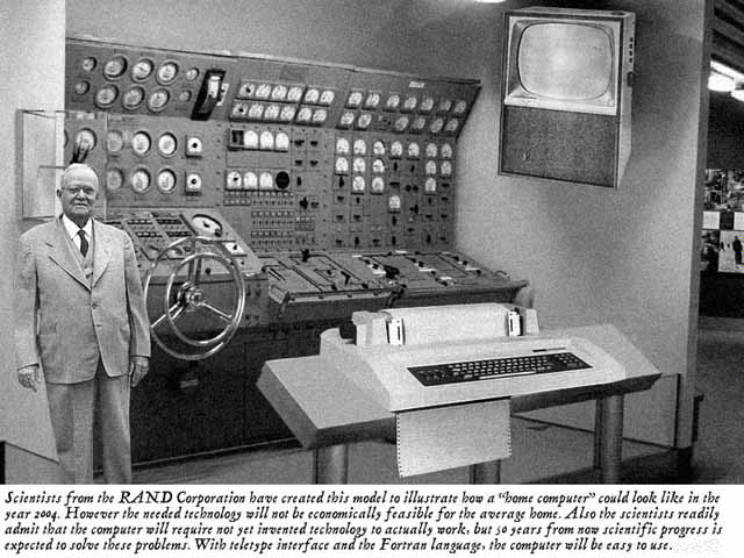
\includegraphics[width=0.9\linewidth]{figures/old-computer.jpg}}
% --- end paragraph admon ---



% !split
\subsection*{An important observation and a  question}

% --- begin paragraph admon ---
\paragraph{}

The basic tools for mathematical calculations have changed radically.

\textbf{How does this influence science education?}

\begin{itemize}
\item Modern industry and technology is impossible without mathematics and science

\item Weather forecasting, product design, film production, materials science, cellular phones, iPad, lunar missions, GPS, furniture production and much more
\end{itemize}

\noindent
% --- end paragraph admon ---




% !split
\subsection*{Reality}

% --- begin paragraph admon ---
\paragraph{}

\begin{itemize}
\item Students hear about the relevance of the sciences

\item But this relevance is hardly visible in school or the first few years at university

\item Much emphasis on renewal of the wrapping of science, little on the content
\end{itemize}

\noindent
% --- end paragraph admon ---




% !split
\subsection*{Principles}

% --- begin paragraph admon ---
\paragraph{Central aims behind our CSE reform.}

Algorithmic  thinking as a way to

\begin{itemize}
\item Enhance instruction based teaching

\item Introduce Research based teaching  from day one

\item Trigger further insights in math and other disciplines (we need a research program to understand if this is the case)

\item Validation and verification of scientific results (the PRL example), with the possibility to emphasize ethical aspects as well. Version control is central.
\end{itemize}

\noindent
% --- end paragraph admon ---





% !split
\subsection*{Research based teaching}

% --- begin paragraph admon ---
\paragraph{How do we define it?}
One possible definition: It is coupled to a direct participation in actual research and builds upon established
knowledge and insights about scientific methods.


\begin{itemize}
\item It is the standard situation at all universities  and takes normally place at the senior undergraduate/graduate level (isn't it too late?)

\item It is seldom done in undergraduate courses.

\item Taught by a researcher

\item The student starts seeing the countour of the scientific approach leading her/him to make new interpretations, develop new insights and understandings that lead  to further research.
\end{itemize}

\noindent
% --- end paragraph admon ---





% !split
\subsection*{Research based education}

% --- begin paragraph admon ---
\paragraph{What should the education contain?}
The standard situation we meet at an almost daily basis:

\begin{itemize}
\item Theory+experiment+simulation is almost the norm in research and industry

\item To be able to model complex systems with no simple answers on closed form. Solve real problems.

\item Emphasis on insight and understanding of fundamental principles and laws in the Sciences.

\item Be able to visualize, present, discuss, interpret and come with a critical analysis of the results, and develop a sound ethical attitude to own and other's work.
\end{itemize}

\noindent
Our education should reflect this.
% --- end paragraph admon ---





% !split
\subsection*{Research based education}

% --- begin paragraph admon ---
\paragraph{Normal workflow in Science and Engineering.}

\begin{itemize}
\item A problem is properly described using a precise (normal) language.

\item It is translated to a mathematical problem using known laws and  principles.

\item It is solved, normally via numerical similations.

\item The solution is visualized and analyzed.

\item The solution to the problem is formulated.
\end{itemize}

\noindent
People who master these skills bring an important compentence to society.
% --- end paragraph admon ---



% !split
\subsection*{Computers and science teaching}

% --- begin paragraph admon ---
\paragraph{Education.}

\begin{itemize}
\item During the  last 25 years  there has been considerable focus on  technology at all levels in the educational ladder.

\item Calculators, text processing, email, digital learning environments etc.

\item Much focus on means and technologies, but what about the content, or more importantly, insight into  physical systems?
\end{itemize}

\noindent
The basic topics (math, chemistry, physics, biology etc) are taught more or less in the same fashion as before, unchanged over several decades!
% --- end paragraph admon ---




% !split
\subsection*{More observations}

% --- begin paragraph admon ---
\paragraph{Computation in the Sciences.}

\begin{itemize}
\item Computations as a fundamental tool  to gain new insights

\item Computer simulations can act as  a lab, can save both time and resources 

\item Computations is a central component in modern industry and research in the sciences, spanning almost every field:
\begin{itemize}

 \item Materials science and nanotechnology, weather forecasting, earthquake simulations and forecasting, medical technology, industrial design, design of new computers, the entertainment industry, almost all aspects of our modern society!!
\end{itemize}

\noindent
\end{itemize}

\noindent
% --- end paragraph admon ---




% !split
\subsection*{Large scale simulations}

% --- begin paragraph admon ---
\paragraph{Fluid dynamical simulations central in air industry.  Typical university courses which are taught address the physics of the lower left corner.}


% inline figure
\centerline{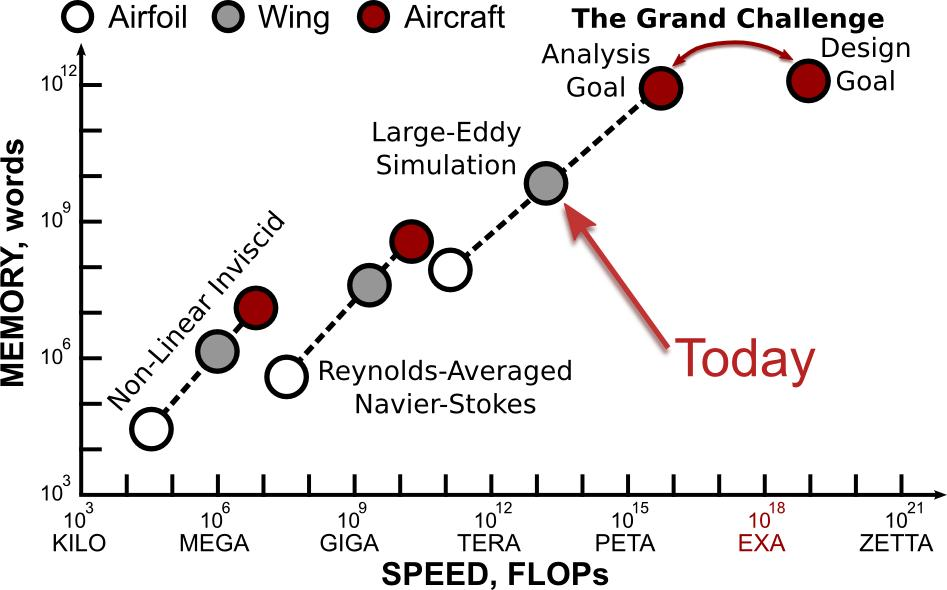
\includegraphics[width=0.6\linewidth]{figures/fig10.jpg}}
% --- end paragraph admon ---




% !split
\subsection*{Large scale simulations}

% --- begin paragraph admon ---
\paragraph{}
Fluid dynamical simulations central in air industry, wings tested.


% inline figure
\centerline{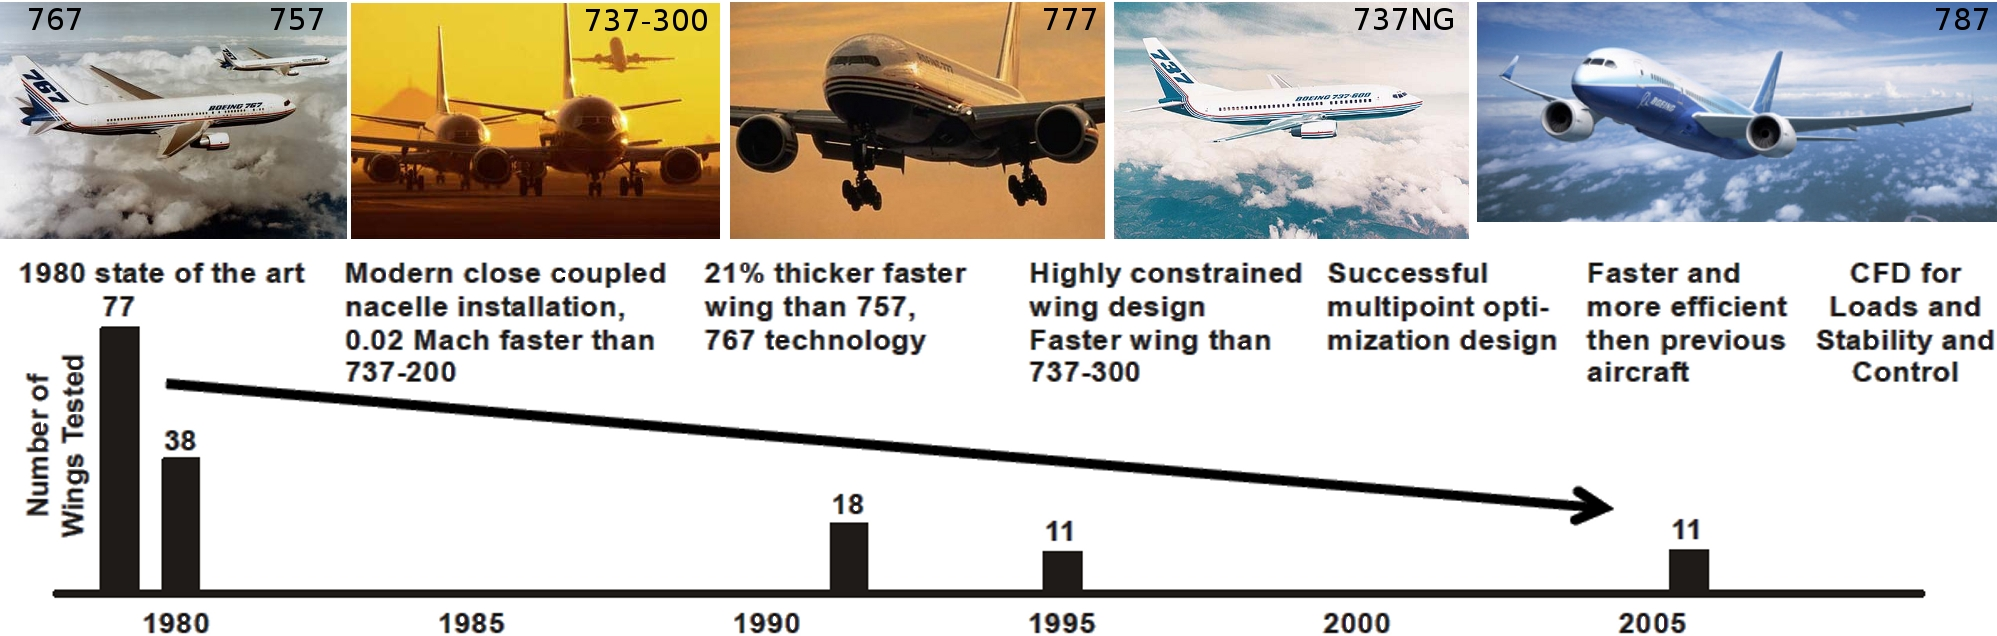
\includegraphics[width=1.0\linewidth]{figures/fig8.jpg}}
% --- end paragraph admon ---




% !split
\subsection*{Nano and macro-scale reactions in rocks}

% --- begin paragraph admon ---
\paragraph{}


% inline figure
\centerline{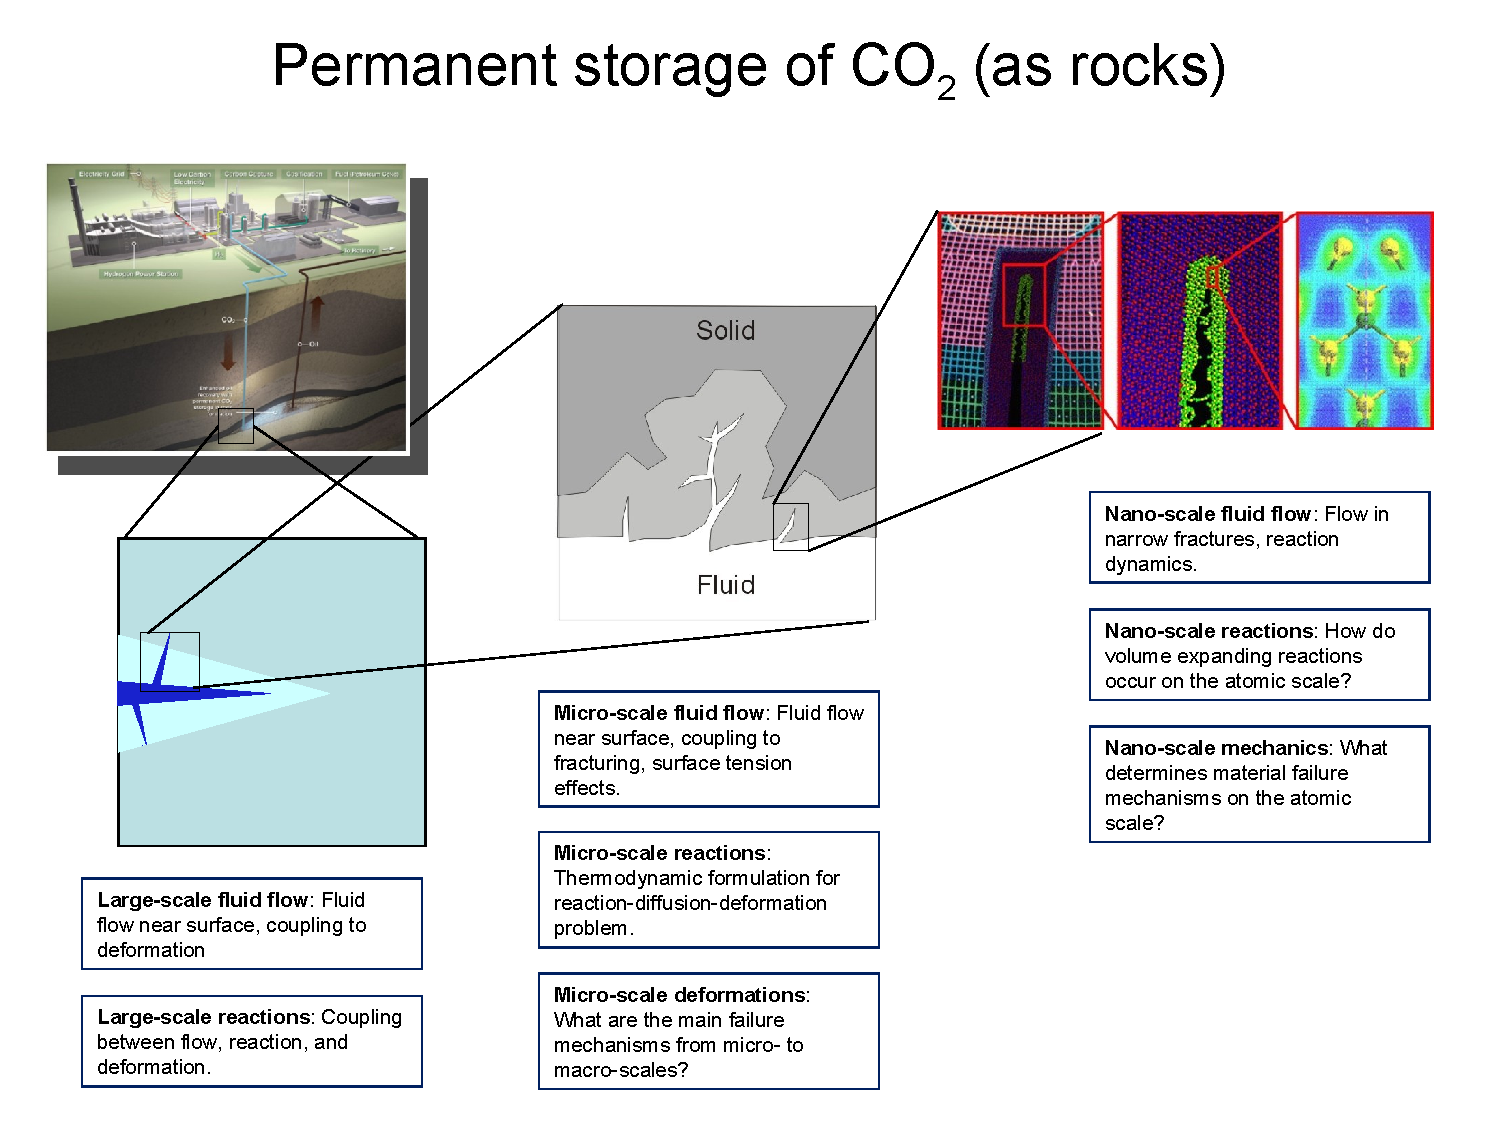
\includegraphics[width=0.8\linewidth]{figures/rocks.pdf}}
% --- end paragraph admon ---





% !split
\subsection*{Further observations}

% --- begin paragraph admon ---
\paragraph{Computations should enter science education.}

\begin{itemize}
\item Our teaching should include  an education in basic numerical methods, normally taught in different departments, and often disconnected. 

\item The students should also learn to develop new methods and learn new tools when needed.

\item Need an adequate computational platform.
\end{itemize}

\noindent
% --- end paragraph admon ---





% !split
\subsection*{More observations}

% --- begin paragraph admon ---
\paragraph{Observations about implementations.}

\begin{itemize}
\item One creates different physics courses and graduate programs which bake in computations, typically various Computational Physics courses from sophomore to graduate level.  The problem is that these courses are not compulsory. The result is often an uneven background of the students. 

\item Dedicated teachers incorporate numerical exercises (at different levels) in their physics courses. When new teachers take over, the whole initiative may disappear. 

\item Some  physics departments in Europe teach their own math and computer science courses! But have still not been able to coordinate properly computational topics.
\end{itemize}

\noindent
% --- end paragraph admon ---




% !split
\subsection*{Can we catch many birds with one stone?}

% --- begin paragraph admon ---
\paragraph{}
\begin{itemize}
\item How can we include and integrate an algorithmic (computational) perspective   in our basic education?

\item Can this enhance the students' understanding of mathematics and science?

\item Can it strengthen research based teaching?
\end{itemize}

\noindent
% --- end paragraph admon ---




% !split
\subsection*{Preliminary summary}

% --- begin paragraph admon ---
\paragraph{Computations should enter basic science education.}

\begin{itemize}
\item Computation is a fundamental tool to gain new insights and should be included in our elementary teaching.

\item Requires development of algorithmic thinking.

\item Basic numerical methods should be part of the compulsory curriculum.

\item The students should also learn to develop new numerical methods and adapt to new software tools.

\item Requires more training than simple programming in a mathematics course.
\end{itemize}

\noindent
% --- end paragraph admon ---




% !split
\subsection*{What is needed?}

% --- begin paragraph admon ---
\paragraph{Programming.}
A compulsory programming course with a strong mathematical flavour. \emph{Should give a solid foundation in programming as a problem solving technique in mathematics}. Programming is understanding! The line of thought when solving mathematical problems numerically enhances algorithmic thinking,  and thereby the students' understanding of the scientific process.
% --- end paragraph admon ---




% --- begin paragraph admon ---
\paragraph{Mathematics and numerics.}
Mathematics is at least as important as before, but should be supplemented with development, analysis, implementation, verification and validation of numerical methods. Science ethics and better understanding of the pedagogical process, almost for free!
% --- end paragraph admon ---




% --- begin paragraph admon ---
\paragraph{Sciences.}
Training in modelling and problem solving with numerical methods and visualisation, as well as traditional methods in Science courses, Physics, Chemistry, Biology, Geology, Engineering...
% --- end paragraph admon ---





% !split
\subsection*{Implementation}

% --- begin paragraph admon ---
\paragraph{Crucial ingredients.}

\begin{itemize}
\item Support from governing bodies (now priority 1 of the College of Natural Science at UOslo)

\item Cooperation across departmental boundaries

\item Willingness by individuals to give priority to teaching reform
\end{itemize}

\noindent
Consensus driven approach.
% --- end paragraph admon ---





% !split
\subsection*{Implementation in Oslo: The CSE  project}

% --- begin paragraph admon ---
\paragraph{What we do.}
\begin{itemize}
\item Coordinated use of computational exercises and numerical tools in most undergraduate courses.

\item Help update the scientific staff's competence on computational aspects and give support (scientific, pedagogical and financial)  to those who wish to revise  their courses in a computational direction.

\item Teachers get good summer students to aid in introducing computational exercises

\item Develop courses and exercise modules with a computational perspective, both for students and teachers. 

\item Basic idea: mixture of mathematics, computation, informatics and topics from the physical sciences.
\end{itemize}

\noindent
Interesting outcome: higher focus on teaching and pedagogical issues!!
% --- end paragraph admon ---




% !split
\subsection*{Example of bachelor program, astrophysics}

% --- begin paragraph admon ---
\paragraph{}


% inline figure
\centerline{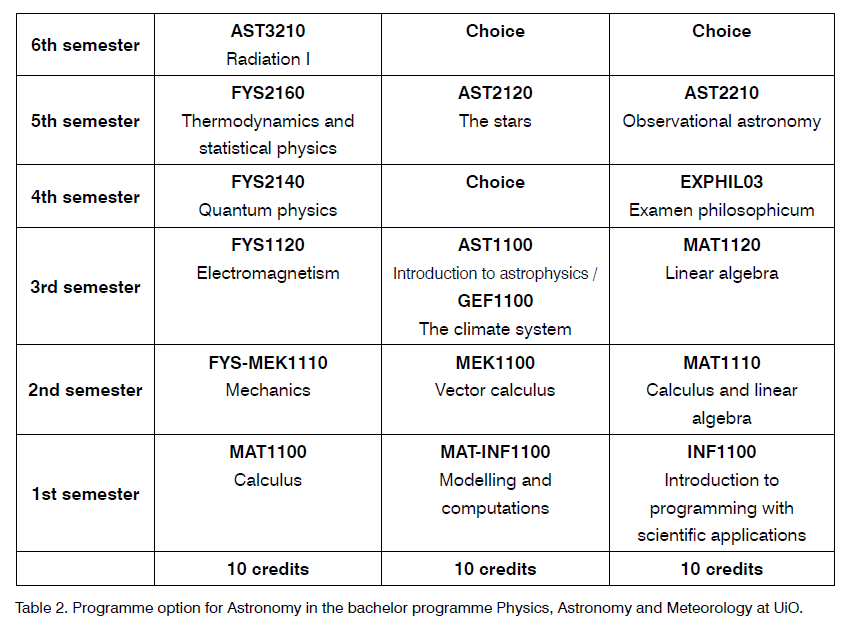
\includegraphics[width=0.6\linewidth]{figures/astronomy.png}}
% --- end paragraph admon ---




% !split
\subsection*{Example: Computations from day one}

% --- begin paragraph admon ---
\paragraph{Differentiation.}
Three courses the first semester:  MAT1100, MAT-INF1100 og INF1100.
\begin{itemize}
\item Definition  of the derivative in  MAT1100 (Calculus and analysis) 
\end{itemize}

\noindent
\[
 f'(x)=\lim_{h \rightarrow 0}\frac{f(x+h)-f(x)}{h}.
\]
\begin{itemize}
\item Algorithms to compute the derivative in MAT-INF1100  (Mathematical modelling with computing)
\end{itemize}

\noindent
\[
 f'(x)= \frac{f(x+h)-f(x-h)}{2h}+O(h^2).
\]
\begin{itemize}
\item Implementation in Python in INF1100
\end{itemize}

\noindent
\begin{minted}[fontsize=\fontsize{9pt}{9pt},linenos=false,mathescape,baselinestretch=1.0,fontfamily=tt,xleftmargin=7mm]{python}
def differentiate(f, x, h=1E-5):
     return (f(x+h) - f(x-h))/(2*h)
\end{minted}
% --- end paragraph admon ---



% !split
\subsection*{Example: Computations from day one}

% --- begin paragraph admon ---
\paragraph{Differentiation and comparison with symbolic expressions.}
Combined with the possibility of symbolic calculations with \emph{Sympy}, Python offers an environment where students and teachers alike can test many different aspects of mathematics and numerical mathematics, in addition to being able to verify and validate their codes. The following simple example shows how to extend the simple function for computing the numerical derivative with the possibility of obtaining the closed form or analytical expression
\begin{minted}[fontsize=\fontsize{9pt}{9pt},linenos=false,mathescape,baselinestretch=1.0,fontfamily=tt,xleftmargin=7mm]{python}
def differentiate(f, x, h=1E-5, symbolic=False):
    if symbolic:
        import sympy
        return sympy.lambdify([x], sympy.diff(f, x))
    else:
        return (f(x+h) - f(x-h))/(2*h)
\end{minted}
% --- end paragraph admon ---





% !split
\subsection*{Other Examples}

% --- begin paragraph admon ---
\paragraph{Integration by Trapezoidal Rule.}

\begin{itemize}
\item Definition of integration  in MAT1100 (Calculus and analysis).

\item The algorithm for computing the  integral vha the Trapezoidal rule for an interval $x \in [a,b]$
\end{itemize}

\noindent
\[
  \int_a^b(f(x) dx \approx \frac{1}{2}\left [f(a)+2f(a+h)+\dots+2f(b-h)+f(b)\right] 
\]
\begin{itemize}
\item Taught   in MAT-INF1100  (Mathematical modelling)

\item The algorithm is then implemented in  INF1100 (programming course).
\end{itemize}

\noindent
% --- end paragraph admon ---



% !split
\subsection*{Typical implementation in INF1100}

% --- begin paragraph admon ---
\paragraph{Integration by Trapezoidal Rule.}

\begin{minted}[fontsize=\fontsize{9pt}{9pt},linenos=false,mathescape,baselinestretch=1.0,fontfamily=tt,xleftmargin=7mm]{python}
from math import exp, log, sin
def Trapez(a,b,f,n):
   h = (b-a)/float(n)
   s = 0
   x = a
   for i in range(1,n,1):
       x = x+h
       s = s+ f(x)
   s = 0.5*(f(a)+f(b)) +s
   return h*s

def f1(x):
    return exp(-x*x)*log(1+x*sin(x))

a = 1;  b = 3; n = 1000
result = Trapez(a,b,f1,n)
print result
\end{minted}
% --- end paragraph admon ---




% !split
\subsection*{Typical implementation in INF1100}

% --- begin paragraph admon ---
\paragraph{Symbolic calculations and numerical calculations in one code!}
Python offers an  extremely versatile programming  environment, allowing for the inclusion of analytical studies in a numerical program. Here we show another example
where \emph{SymPy} is used to evaluate the integral and compute the absolute error 
with respect to the numerically evaluated one of the integral
$\int_0^1 dx 4/(1+x^2) = \pi$: 
\begin{minted}[fontsize=\fontsize{9pt}{9pt},linenos=false,mathescape,baselinestretch=1.0,fontfamily=tt,xleftmargin=7mm]{python}
from math import *
from sympy import *
def Trapez(a,b,f,n):
   h = (b-a)/float(n)
   s = 0
   x = a
   for i in range(1,n,1):
       x = x+h
       s = s+ f(x)
   s = 0.5*(f(a)+f(b)) +s
   return h*s

#  function to compute pi
def function(x):
    return 4.0/(1+x*x)

a = 0.0;  b = 1.0; n = 100
result = Trapez(a,b,function,n)
print "Trapezoidal rule=", result
# define x as a symbol to be used by sympy
x = Symbol('x')
exact = integrate(function(x), (x, 0.0, 1.0))
print "Sympy integration=", exact
# Find relative error
print "Relative error", abs((exact-result)/exact)
\end{minted}
% --- end paragraph admon ---




% !split
\subsection*{Integrating numerical mathematics with calculus}

% --- begin paragraph admon ---
\paragraph{}
The last example shows the potential of combining numerical algorithms with symbolic calculations, allowing thereby students and teachers to

\begin{itemize}
\item Validate and verify  their  algorithms. 

\item Including concepts like unit testing, one has the possibility to test and validate several or all parts of the code.

\item Validation and verification are then included \emph{naturally} and one can develop a better attitude to what is meant with an enthically sound scientific approach.

\item The above example allows the student to also test the mathematical error of the algorithm for the trapezoidal rule by changing the number of integration points. The students get trained from day one to think error analysis. 

\item With an ipython notebook the students can keep exploring similar examples and turn them in as their own notebook. 
\end{itemize}

\noindent
% --- end paragraph admon ---






% !split
\subsection*{Learning outcomes three first semesters}

% --- begin paragraph admon ---
\paragraph{Knowledge of basic algorithms.}

\begin{itemize}
\item Differential equations: Euler, modified Euler and Runge-Kutta methods (first semester)

\item Numerical integration: Trapezoidal and Simpson's rule, multidimensional integrals (first semester)

\item Random numbers, random walks, probability distributions and Monte Carlo integration  (first semester)

\item Linear Algebra and eigenvalue problems: Gaussian elimination, LU-decomposition, SVD, QR, Givens rotations and eigenvalues, Gauss-Seidel. (second and third semester)

\item Root finding and interpolation etc. (all three first semesters)

\item Processing of sound and images (first semester).
\end{itemize}

\noindent
The students have to code several of these algorithms during the first three semesters.
% --- end paragraph admon ---




% !split
\subsection*{Later courses}

% --- begin paragraph admon ---
\paragraph{}

\textbf{Later courses should build on this foundation as much as possible}.

\begin{enumerate}
\item In particular, the course should not be too basic! There should be progression in the use of mathematics, numerical methods and programming, as well as science.

\item Computational platform: Python, fully object-oriented and allows for seamless integration of c++ and Fortran codes, as well as Matlab-like programming environment. Makes it easy to parallelize codes as well.
\end{enumerate}

\noindent
% --- end paragraph admon ---



% !split
\subsection*{Coordination}

% --- begin paragraph admon ---
\paragraph{}
\begin{itemize}
\item Teachers in other courses need therefore not use much time on numerical tools. Naturally included in other courses.
\end{itemize}

\noindent
% --- end paragraph admon ---





% !split
\subsection*{FYS-MEK1100 (Mechanics), Second Semester}

% --- begin paragraph admon ---
\paragraph{Realistic Pendulum.}

Classical pendulum with damping and external force
\[
  ml\frac{d^2\theta}{dt^2}+\nu\frac{d\theta}{dt}  +mgsin(\theta)=Asin(\omega t).
\]
Easy to solve numerically without classical simplification, and then visualize the solution.  Done in first semester!
Same equation for an RLC circuit 
\[
L\frac{d^2Q}{dt^2}+\frac{Q}{C}+R\frac{dQ}{dt}=V(t).
\]
% --- end paragraph admon ---




% !split
\subsection*{FYS1120 Electromagnetism, Third Semester}

% --- begin paragraph admon ---
\paragraph{RLC circuit.}
Same equation as the pendulum for an RLC circuit 
\[
L\frac{d^2Q}{dt^2}+\frac{Q}{C}+R\frac{dQ}{dt}=V(t).
\]
From the numerics, 
the students found the optimal parameters for studying experimentally chaos
in an RLC circuit. Then they did the experiment.
% --- end paragraph admon ---






% !split
\subsection*{What can we do with the pendulum?}

% --- begin paragraph admon ---
\paragraph{Many interesting problems.}

\begin{enumerate}
\item Can study chaos, theoretically, numerically and experimentally, can choose 'best' parameters  for experimental setup.

\item Can test different algorithms for solving ordinary differential equations, from Euler's to fourth-order Runge Kutta methods. Tight connection with algorithm and physics.

\item Can make classes of differential equation solvers.

\item Can make a general program that can be applied to other scientific cases in later courses, such as electromagnetism (RLC circuits).  Students realize that much of the same mathematics enters many physics cases.
\end{enumerate}

\noindent
% --- end paragraph admon ---




% !split
\subsection*{More Examples from Physics Courses, 2-5 semester}

% --- begin paragraph admon ---
\paragraph{Second-fourth semester.}

\begin{itemize}
\item Air resistance in two and three dimensions with quadratic velocity dependence.

\item Launching a probe into a tornado

\item Rocket launching with realistic parameters, gravity assist

\item How to kick a football and model its trajectory.

\item Planet motion and position of planets

\item Magnetic fields with various geometries based on Biot-Savart's law

\item Harmonic oscillations and various forms of electromagnetic waves.

\item Combined effect of different potentials such as the electrostatic potential and the gravitational potential.

\item Simple studies of atoms and molecules, and much more
\end{itemize}

\noindent
% --- end paragraph admon ---



% !split
\subsection*{First computational physics course}

% --- begin paragraph admon ---
\paragraph{Late: Fifth semester, FYS3150 Computational Physics.}

The first computational physics \href{{http://www.uio.no/studier/emner/matnat/fys/FYS3150/h14/}}{course} can then be used to summarize many of the gained insights about algorithms, mathematical models, physics etc. And direct the students to more advanced algorithms and applications like

\begin{itemize}
\item Monte carlo methods

\item Parallelization

\item Solving quantum mechanical problems by Variational Monte Carlo  or other quantum mechanical methods

\item Study phase transitions with for example the Ising and Potts model.

\item Molecular dynamics simulations etc etc 
\end{itemize}

\noindent
% --- end paragraph admon ---




% !split
\subsection*{Challenges...}

% --- begin paragraph admon ---
\paragraph{.. and objections.}

\emph{Standard objection: computations take away the attention from other central topics in 'my course'}. 

CSE incorporates computations from day one, and courses higher up do not need to
spend time on computational topics  (technicalities), but can focus on the interesting
science applications.

\begin{itemize}
\item To help teachers: Developed pedagogical modules which can aid university teachers.
\end{itemize}

\noindent
% --- end paragraph admon ---



% !split
\subsection*{Challenges and future plans}

% --- begin paragraph admon ---
\paragraph{}

\begin{itemize}
\item The project depends crucially on few individuals. 

\item Need to get more teachers involved, not only good TAs.

\item How  to implement a CSE perspective in other programs like Chemistry, Molecular Biology,  Biology, Engineering. New courses are being developed.

\item Now a national pilot for other universities and regional colleges.
\end{itemize}

\noindent
\textbf{Key issue: modularization of topics and development of a 'technological platform' which glues together different modules}
% --- end paragraph admon ---



% !split
\subsection*{Which aspects are important for a successful introduction of CSE?}

% --- begin paragraph admon ---
\paragraph{}

\begin{itemize}
\item Early introduction, programming course at beginning of studies linked with math courses and science and engineering courses.

\item Crucial to learn proper programming at the beginning.

\item Choice of software.

\item Textbooks and modularization of topics.

\item Resources and expenses.

\item Tailor to specific disciplines.

\item Organizational matters.
\end{itemize}

\noindent
% --- end paragraph admon ---



% !split
\subsection*{Do we get better students?}

% --- begin paragraph admon ---
\paragraph{Molecular dynamics visualization by two MSc students.}


% inline figure
\centerline{\includegraphics[width=0.7\linewidth]{figures/visualize.jpg}}



% \includegraphics[width=9.5cm]{visualize.jpg}
% --- end paragraph admon ---




% !split
\subsection*{Summary}

% --- begin paragraph admon ---
\paragraph{}

\begin{itemize}
\item Make our research visible in early undergraduate courses, enhance research based teaching

\item Possibility to focus more on understanding and increased insight.

\item Impetus for broad cooperation in teaching.

\item Strengthening of instruction based teaching (expensive and time-consuming).

\item Give our candidates a broader and more up-to-date education with a problem-based orientation, often requested by potential employers.

\item And perhaps the most important issue: does this enhance the student's insight in the Sciences?
\end{itemize}

\noindent
% --- end paragraph admon ---





% ------------------- end of main content ---------------


\printindex

\end{document}

